\documentclass[a4paper,oneside]{scrarticle}

\usepackage[left=3cm,right=3cm,top=2cm,bottom=2.25cm]{geometry}
\usepackage[ngerman]{babel}
\usepackage{amsmath}
\usepackage{amsfonts}
\usepackage{amssymb}
\usepackage{mathtools}
\usepackage{graphicx}\usepackage{hyperref}
\usepackage{fancyhdr}
\addto\captionsngerman{\renewcommand{\figurename}{Fig.}}


\begin{document}
	% Set the page style to "fancy"...
	\pagestyle{fancy}
	%... then configure it.
	\fancyhead{} % clear all header fields
	\fancyhead[L]{Bach Nguyen, Johannes Roloff - HTWK Leipzig - INB}
	\fancyfoot{} % clear all footer fields
	\begin{center}
		\begin{LARGE}
			\textbf{Station 3 Reflexion}
		\end{LARGE}
	\end{center}
	
	\section*{Einordnung der Aufgabe im Prozess}
	\begin{figure} [h]
		\centering
		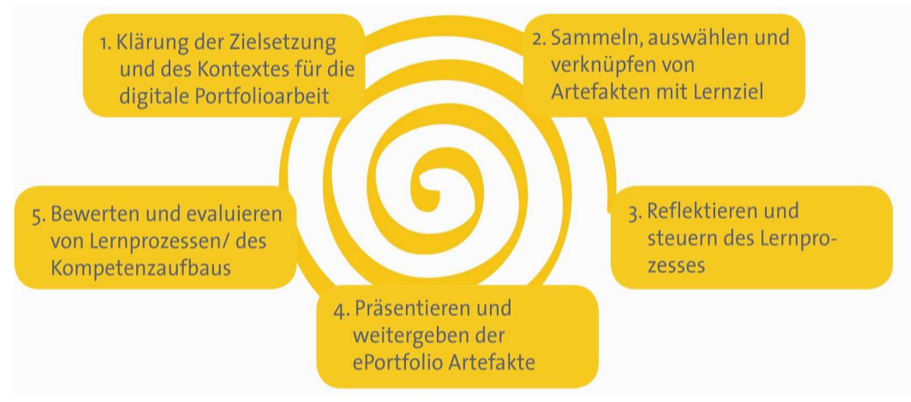
\includegraphics[width=0.7\linewidth]{e-portfolio-prozesse-schaffert}
		\caption{Prozesse der Portfolio-Arbeit (Schaffert et al. 2007, S. 79)\cite{schaffert_e-portfolio-einsatz_2007}}
		\label{fig:e-portfolio-prozesse-schaffert}
	\end{figure}
	\begin{figure}[h]
		\centering
		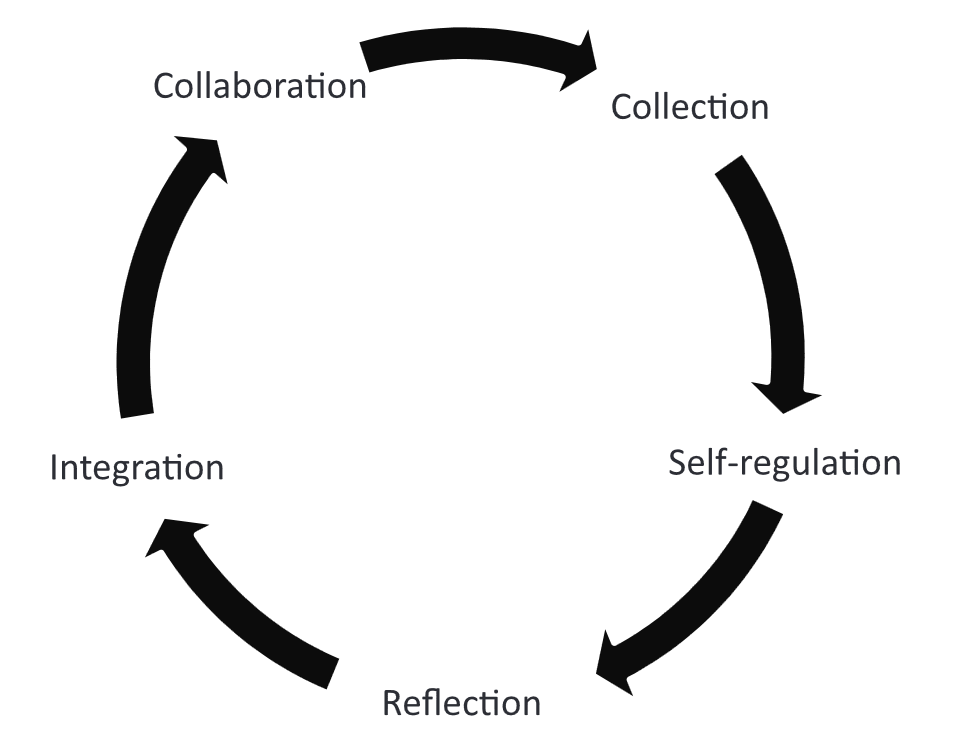
\includegraphics[width=0.5\linewidth]{cycle-of-documented-lifelong-learning-Jensen}
		\caption{cycle of documented lifelong learning (Jensen,Treuer 2014)\cite{jenson_defining_2014}}
		\label{fig:cycle-of-documented-lifelong-learning-jensen}
	\end{figure}
	\begin{figure}[h]
		\centering
		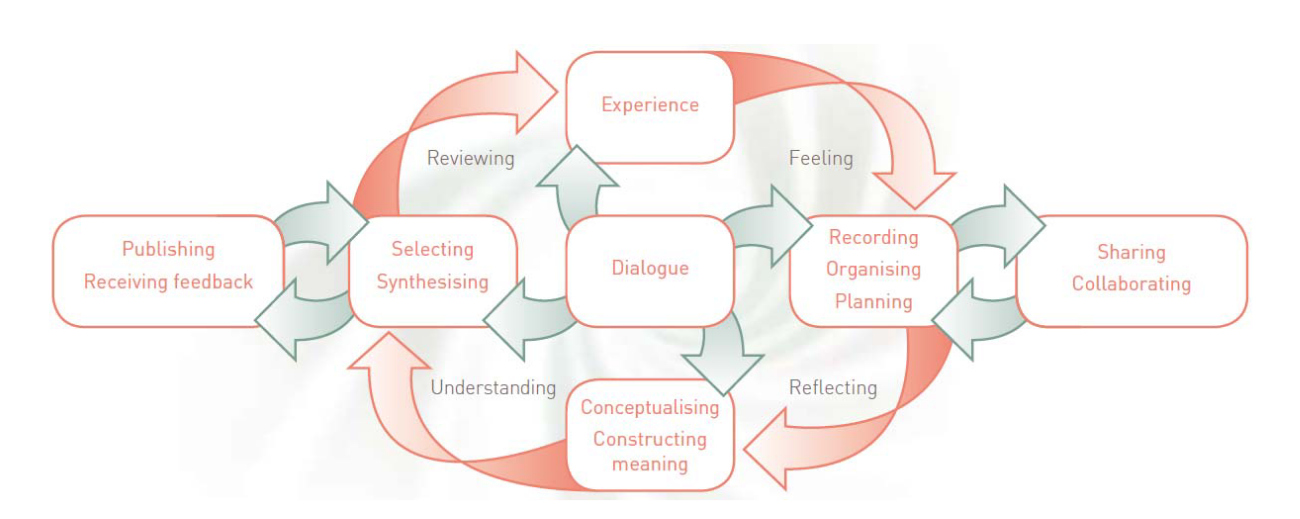
\includegraphics[width=0.8\linewidth]{model-of-e-portfolio-based-learning}
		\caption{A model of e-portfolio-based learning (JISC 2008, S. 9) \cite{jisc_effective_2008}}
		\label{fig:model-of-e-portfolio-based-learning}
	\end{figure}
	
	\pagebreak 
	
	\section*{Informationsmaterialien}
	
	Belese dich zu den Qualitäten der \href{https://doi.org/10.1007/s40692-020-00157-6}{Reflexion}\cite{sultana_e-portfolios_2020} und versuche nachzuvollziehen, wie die Reflexion dich in deinem eigenen Lernen unterstützen kann.\\
	Bewerte die 6 Stufen auf der 	\href{https://sci-hub.ru/https://www.tandfonline.com/doi/epdf/10.1207/s15430421tip4104_2?needAccess=true}{Bloom's Taxonomy} \cite{krathwohl_revision_2002}, indem du sagst, ob du übereinstimmst.
	
	
	\bibliographystyle{alpha}
	\bibliography{../eportfolio_lib}
	
	\pagebreak
	
	\section*{Einleitung}
	Was bedeutet Reflexion und was bedeutet Selbstreflexion? Lohnt es sich einen Blick nochmal auf dein Lernverhalten zu werfen? Gibt es unterschiedliche Stufen von Selbstreflexion?
	
	\section*{Aufgabenstellung}

	\begin{enumerate}
		\item Versetze dich nun in die Lage, jetzt mitten im Semester zu sein. Nehme dir zu erst deine Lernziele, die du in Station 1 erarbeitet hast und analysiere, ob du auf einem guten Weg bist, diese zu erreichen. Folgende Fragen sollen dich hierbei unterstützen. Schreibe dazu einen Selbstreflexionsbericht 
		\begin{enumerate}
			\item Bin ich zufrieden mit meiner bisherigen Lernleistung?
			\item Sind meine Ziele immer noch SMART, muss ich sie anpassen?
			\item Was sind die größten Probleme auf die ich gestoßen bin?
			\item Habe ich neue Stärken und Schwächen an meinem Lernen entdeckt?
			\item Wie kann ich meine Stärken noch besser Nutzen?
			\item Wie kann ich meine Defizite beheben?
			\item Was habe ich denn bis jetzt wirklich gelernt?
			\item Macht mir das Lernen Spaß?
			\item Wie könnte ich meine Motivation aufrechterhalten?
			\item Was ist für mich der Sinn, dieses Modul zu machen?
			\item Was hat sich in meiner Einstellung zu diesem Thema fundamental verändert?
			\item Gibt es Dinge, die ich bis zum Ende des Semesters anders machen sollte?
		\end{enumerate}
		\item Weiterführende Fragen mithilfe der Bloom's Taxonomy zur Unterstützung des Schreibens
		\begin{enumerate}
			\item Auf welcher Stufe der Bloom's Taxonomy sehe ich mich im Moment?
			\item Welche Lernmethoden habe ich angewandt?
			\item Wie effektiv waren diese Lernmethoden gewesen?
			\item Welche Stufen der Bloom's Taxonomy wurde mit der jeweiligen Lernmethode angesprochen?
			\item Wie könnte ich mit der jetztigen/oder vielleicht mit einer anderen Methode denn noch ein höheres Level erreichen?
		\end{enumerate}
		\item Schreibe nun einen Reflexionsbericht, über dem ganzen Verlauf Deines bisherigen Studiums. Nehme dir die Fragen aus der Aufgabe 1 und folgende zur Unterstützung.
		\begin{enumerate}
			\item Wie fühlt sich mein Studium für mich momentan an?
			\item Wie sehr haben sich meine Erwartungen an das Studium verändert?
		\end{enumerate}

	\end{enumerate}


\end{document}
